\documentclass[11pt]{article}
\usepackage[a4paper, total={6in, 8in}]{geometry}
\usepackage{amsmath}
\usepackage{amsthm}
\usepackage{graphicx}
\usepackage{amsfonts}
\usepackage{xcolor}
\begin{document}

\newtheorem{theorem}{Theorem}
\numberwithin{theorem}{section}
\theoremstyle{definition}
\newtheorem{definition}{Definition}
\newtheorem{proposition}{Proposition}
\newtheorem{example}{Example}
\newtheorem{lemma}{Lemma}
\newtheorem{corollary}{Corollary}
\numberwithin{definition}{section}
\numberwithin{proposition}{section}
\numberwithin{example}{section}
\numberwithin{lemma}{section}
\numberwithin{corollary}{section}
\newcommand{\uw}{\mathcal{U}(W,X)}
\newcommand{\W}{$(W,S)$}
\newcommand{\ix}{\textit}
\newcommand{\tr}{\textcolor{red}}
\newcommand{\sg}{$\Sigma$}


\title{Shadows in the Wild}
\maketitle
\tableofcontents 



\textcolor{red}{Red notes for Megan}

\textcolor{blue}{Blue notes for Yusra}

\section{Roots}

In this text, we are considering galleries of the form $\gamma=(\lambda_0,c_0,p_1,c_1,...,p_n,c_n,\lambda_n)$, i.e galleries which start and end at vertices. This is slightly different to the other convention of starting and ending at alcoves. This changes the concept of minimla galleries slightly. 

We also take our orientation to be a fixed Weyl chamber orientation. So we have fixed a chamber at infinity which defines the orientation.

\begin{definition}
    Let $\gamma$ be a gallery in a Coxeter complex $\Sigma$. At $p_i$, the hyperplane containing $p_i$ is said to be \ix{load-bearing} if $c_i$ lies on the positive side of the hyperplane. A hyperplane containing $\lambda_0$ is called \ix{load-bearing} if $c_0$ is on the positive side.
\end{definition}

Note that at each panel, we have at most one load-bearing hyperplane, but at the starting vertex we can have multiple. The number of load-bearing hyperplanes at $\lambda_0$ is bounded by the number of hyperplanes in the spherical Weyl group, or equivantely the size of a positive root system defining the Weyl group. 

\begin{definition}
    Given a gallery $\gamma$, its \ix{dimension} is the number of pairs $(p_i,H)$, where $H$ is a load-bearing hyperplane at $p_i$. 
\end{definition}

\begin{definition}
    Given a fixed end-vertex and fixed type $\tau$, a gallery of maximal possible dimension is called a \ix{LS-gallery} of type $\tau$. 
\end{definition}

\tr{Is this related to the $\phi$-valuation? This seems very similar to the dominant alcove but 'the other way round'}

\begin{proposition}
    Let $\gamma$ be an LS-gallery. Then
    \begin{enumerate}
        \item An application of $e_\alpha$ will increase the dimension of $\gamma$ by one.
        \item An application of $f_\alpha$ will decrease the dimension of $\gamma$ by one.
        \item Applying $e_\alpha$ then $f_\alpha$ gives the original gallery $\gamma$. Applying $f_\alpha$ then $e_\alpha$ gives the original gallery $\gamma$.
        \item The set of LS-galleries is closed under applying e and f operators.
        \item Any LS-gallery of the same type as $\gamma$ can be formed from $\gamma$ by a finite number of $e$ and $f$ operators.
    \end{enumerate}
\end{proposition}

\tr{How can this proposition be true when LS-galleries are defined to be the maximal dimension galleries of a certain type, and I don't think $e$ and $f$ will change the type.}

\begin{proposition}
    Let $\lambda$ be a dominant vertex in \sg. Let $\phi$ be the Weyl chamber orientation which is induced by the anti-dominant Weyl chamber. Then we have
    \[\textnormal{Sh}_\phi^\vee (\lambda)=\{\nu \leq \lambda|\nu \textnormal{ is a vertex with the same type as }\lambda\}.\]
\end{proposition}

\tr{Is the ordering here Bruhat ordering?}

\begin{definition}
    Let $A$ be a chosen apartment in a building $X$, and let $c\in A$ be an alcove. We define the \ix{retraction from X to A based at c} as the map $r_{A,c}:X\longrightarrow A$ where we send any alcove $d$ to its image under the isomorphism from the apartment containing both $c$ and $d$ to $A$. 
\end{definition}

\tr{How do we know that this isomorphism is unique?}\\
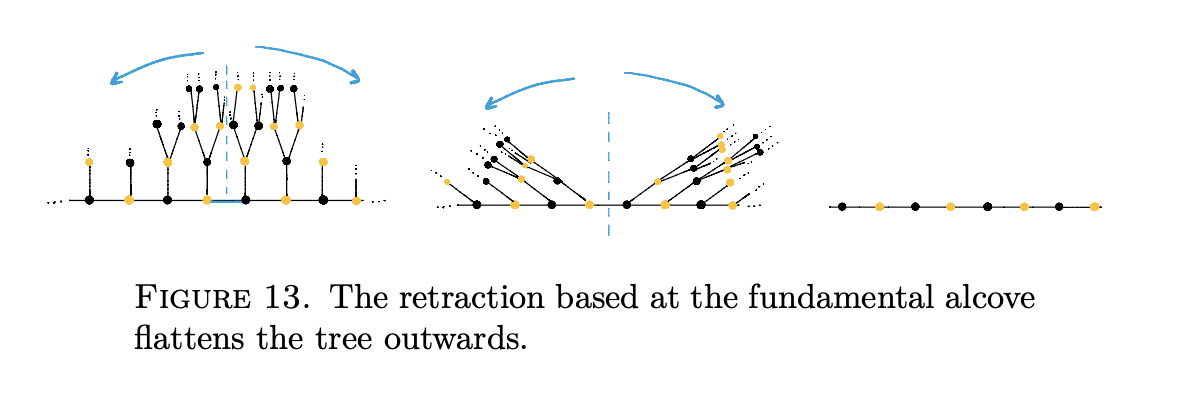
\includegraphics[scale=0.6]{Screenshot 2023-02-15 at 13.32.45.png}
\begin{definition}
    Let $A$ be a chosen apartment in an affine building $X$, and let $C\in \partial A$ be a chamber at infinity of the apartment. We define the \ix{retraction from X to A based at C} as the map $\rho_{A,C}:X\longrightarrow A$, which sends an alcove $d$ to its image under the isomorphism from the apartment containing both $d$ and a Weyl chamber representing $C$ to $A$. 
\end{definition}


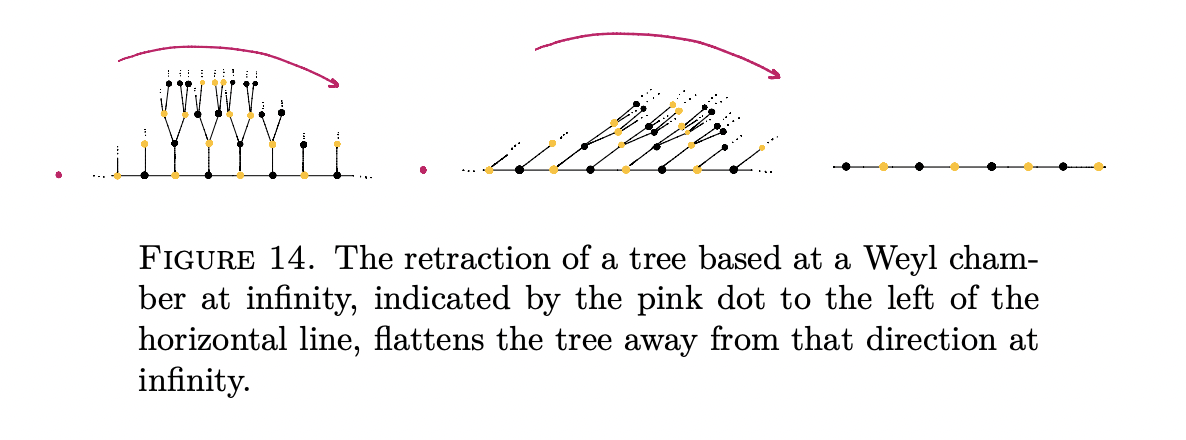
\includegraphics[scale=0.6]{Screenshot 2023-02-15 at 13.31.58.png}


\section{Kostant Convexity}

\begin{theorem}
    We note that we can decompose any reductive group $G$ with assiciated Bruhat-Tits building as
    \[G=UTK,\]
    where $U$ is the stabiliser of the parallel class of the anti-dominant Weyl chamber in the base apartment $A_0$, $T$ is the set of translations of $A_0$, and $K$ is the stabiliser of the origin on $A_0$. 
    Then for all $t,t'\in T$, we have
    \[Ut'K\cap KtK\neq \emptyset \iff t'K\in\textnormal{conv}(W_0\cdot tK).\]
\end{theorem}


\begin{theorem}
    Consider a thick affine building $X$, with fixed base apartment $A_0$ with origin $\lambda_0$, base alcove $c_0$ and fundamental Weyl chamber $C_0$. Choose a special vertex $\lambda$ in $a_0$. Then,
    \[\rho_{C_0,A}(r^{-1}_{c_0,A}(W_0\cdot\lambda))=\textnormal{conv}(W_0\cdot \lambda).\]
\end{theorem}


\section{Affine Deligne-Lusztig varieties}

Let $F=k((t))$, where $k$ is the algebraic closure of the finite field of order $q=p^m$, where $p$ is prime. Let $\sigma$ be the Frobenius map of $\mathbb{F}_q$. We denote by $\mathcal{O}$ the ring of integers $k[[t]]$. 


\begin{definition}
    Let $G$ be a connected reductive group over $\mathbb{F}_q$. The quotient $G(F)/I$ is called the 
\end{definition}


























\end{document}